\documentclass[12pt]{report}
\usepackage{setspace}  %use this package to set linespacing as desired
\usepackage{array}
\usepackage{graphicx}
\usepackage{subcaption}
\usepackage{amsmath}
\usepackage{color,soul}
\usepackage[counterclockwise, figuresleft]{rotating}

\begin{document}
\doublespacing

\clearpage
\chapter{Background and Motivation}

%%%
\section{Shadow Removal}
%%%

\subsection{History}

\hl{Shadow removal is a necessary step in correct segmentation of foreground objects for proper tracking, as shadows are often brought into the foreground of scene processed with traditional background modeling [3, 4]. A taxonomy of shadow removal methods produced by Prati et al. summarizes and evaluates four contemporary method classes: Statistical Nonparametric, Statistical Parametric, Deterministic Nonmodel-based and Deterministic Nonmodel-based 2 [2]. The study concluded that the simpler methods were more suited for general practice, but “to detect shadows efficiently in one specific environment, [adding] more assumptions yield better results.” A second algorithm survey conducted by Sanin et al. in [1] evaluated more modern methods (catalogued as Chromacity, Geometry, Physical, Small Region Texture, and their own contribution, Large Region Texture) on the same datasets as above, yielding similar results concerning the generalization of shadow removal to an arbitrary scene. Our proposed research uses the same datasets as the two surveys. Mitra et al. provides a survey of threshold selection strategies for identifying shadows in moving foreground objects [3].}

\textit{Add blurbs about foreground, background, cast shadows, images.}

\subsubsection{Evaluation Metrics}

The efficacy of a shadow removal algorithm on a frame is evaluated with the popular metrics \textit{Detection} ($\eta$) and \textit{Discrimination} ($\xi$) (Eqn. \ref{eqn:detection}, Eqn. \ref{eqn:discrimination}). These formulae measure how many shadow pixels are correctly identified, and how many foreground object pixels are correctly preserved, respectively. The metrics are calculated using true positives (TP) and false negatives (FN) of both foreground pixels and shadow pixels. Subscripts represent either (s)hadow pixels or (f)oreground pixels.

\begin{equation}
\eta = \dfrac{TP_{S}}{TP_{S} + FN_{S}} \label{eqn:detection}
\end{equation}

\begin{equation}
\xi = \dfrac{TP_{F}}{TP_{F} + FN_{F}} \label{eqn:discrimination}
\end{equation}

\subsection{Shadow Removal Methods} \label{section:removalmethods}

Standardized implementations of popular shadow removal methods, including ground truths, backgrounds, and frames, are used courtesy of A. Sanin, C. Sanderson, B.C. Lovell (http://arma.sourceforge.net/shadows), licensed under GPL v3+ and written in C++.

\subsubsection{Chromacity}

\textit{Chromacity}, or \textit{hue}, represents the base color of a pixel, and is separable from brightness and saturation. Chromacity-based shadow removal methods maintain that a pixel, when covered by a shadow, loses luminosity (or brightness), while retaining its chromacity. This assumption is referred to as  color constancy, or linear attenuation. This study implements one such algorithm from Cucchiara et al. [\ref{gucciara}], implemented using the Hue-Saturation-Value (HSV) color representation. 

Cucchiara et al. observe a shadowed pixel in the foreground ($fg_{p}$) retains its hue when compared to the corresponding background pixel ($bg_{p}$), while losing saturation and intensity (value). In order to be considered a shadow, the hue, saturation, and value of $fg_{p}$ must fall within the pre-determined thresholds $\tau_{H}$, $\tau_{S}$, and [$\beta_{1}$, $\beta_{2}$] (Eqn. \ref{eqn:huethresh}, \ref{eqn:satthresh}, \ref{eqn:brightthresh}).

\begin{equation} \label{eqn:huethresh}
| fg_{p}(H) - bg_{p}(H) | \leq \tau_{H}
\end{equation}

\begin{equation} \label{eqn:satthresh}
fg_{p}(S) - bg_{p}(S) \leq \tau_{S}
\end{equation}

\begin{equation} \label{eqn:brightthresh}
\beta_{1} \leq \dfrac{fg_{p}(V)}{bg_{p}(V)} \leq \beta_{2}
\end{equation}

The thresholds are optimized for the environment the algorithm is intended to be deployed to. Due to its reliance on curated thresholds, Chromacity shadow removal is sensitive to strong illumination changes. Furthermore, the assumed linear attenuation model performs worse with dark shadows. 

\subsubsection{Physical}

For a shadow pixel to attenuate linearly, the light source casting the shadow must consist of primarily white light. Many environments experience multiple light sources, whether they are the sun, surface reflections, or blue light refracted from the sky. The presence of non-white light sources causes non-linear attenuation from a foreground shadow pixel to its background pixel.

This study uses an implementation of Cheng et al.'s Physical shadow removal, which attempts to learn the attenuation model of a shadow using a Gaussian Mixture Model (GMM) [\ref{Phys}]. Three features are used to learn the attenuation model of a pixel ($p$): illumination attenuation ($\alpha_{p}$), red-green direction ($\theta_{p}$), and blue direction ($\phi_{p}$). $\theta_{p}$ and $\phi_{p}$ are spherical coordinates, derived from the representation of the pixel $p$ as a vector $\vec{v}_{p}$ in the RGB coordinate plane. $\vec{bg}_{p}$ represents the pixel vector associated with the corresponding background model. Eqn. \ref{eqn:alphaatten}, Eqn. \ref{eqn:rgangle}, and Eqn. \ref{eqn:bangle} describe the calculation of these features.

\begin{equation} \label{eqn:alphaatten}
\alpha_{p} = \dfrac{||\vec{v}_{p}||}{||\vec{bg}_{p}||}
\end{equation}

\begin{equation} \label{eqn:rgangle}
\theta_{p} = arctan(\dfrac{\vec{v}_{p}(G)}{\vec{v}_{p}(R)})
\end{equation}

\begin{equation} \label{eqn:bangle}
\phi_{p} = arccos(\dfrac{\vec{v}_{p}(B)}{||\vec{v}_{p}||})
\end{equation}

Physical shadow removal first uses a weak detector to identify candidate shadow pixels, calculates the appropriate color features, and uses them to update the GMM. The GMM learns the attenuation model of a shadow over time, and is used to discriminate between foreground object pixels and shadow pixels.

\subsubsection{Geometry}

Popular Geometry-based shadow removal methods attempt to identify shadow regions in a foreground object using projective geometry [\ref{from sanin, mulitple}]. The implementation evaluated in this study, proposed by Hsieh et al. [\ref{Hsieh}], characterizes the geometric moments of foreground blobs in an attempt to identify the vertical peak and center of gravity of the objects. Using this information, the foreground object is split into an object region and a shadow region.

Geometric removal methods often require a shadow and an object retain a clear orientation in regard to one another. Geometric removal is best deployed in environments with distinct, upright objects with a strong directional source of light.  

\subsubsection{Small-Region Texture}

Texture-based shadow removal attempts to match shadow pixels based on the underlying background texture, i.e., structural patterns observed in both the background model and the foreground. If similar structural patterns are observed, it is concluded that the foreground region does not occlude the background, and is therefore more likely to be a cast shadow.

Small-Region Texture (SRT) shadow removal, proposed by Leone et al. [\ref{Leone}], utilizes a set of Gabor functions with various bandwidths, orientations, and phases. A set of candidate shadow pixels, determined by a weak detector similar to that of Physical removal, is projected onto the set of Gabor filters. After analyzing both foreground and background, the texture correlation is found by computing the Euclidean distance.

\subsubsection{Large-Region Texture}

Large-Region Texture (LRT) shadow removal recognizes that the small regions analyzed using SRT may fail to contain enough structural information to match foreground to background. LRT takes advantage of Chromacity removal to produce regions of probable shadow candidates, and correlates the gradient information of both the foreground and background regions. LRT removal proves most effective in environments characterized by strong textural features and large contiguous shadow regions.

%The datasets used by Sanin et al. were also provided, and as such will be utilized in this research for more direct and accurate evaluations. The datasets vary in terms of environment, lighting, time of day, and actors of the scene. These different qualities lend themselves to be quite distinct from one another in terms of shadow length, color, orientation, and definition. Four datasets are indoors, and three outdoors. The spatial environments also differ in key factors such as background textures and color variances.

\subsection{Motivation}

%%% This is basically the abstract?
%Object tracking and segmentation are pivotal to most preeminent computer vision applications, ranging in application from security and surveillance, to traffic monitoring and analysis. Notably, many applications utilize the extraction of foreground pixels to capture moving objects in a scene; since shadows share movement patterns with foreground objects (and have a similar magnitude of intensity change compared with the background model), they tend to be extracted alongside the desired object pixels [1]. While this may occasionally be the intention, shadows generally contribute to inaccurate object classifications and impede proper tracking of foreground objects. In order to rectify this, there have been a bevy of developments regarding shadow detection and removal from foreground objects. In order to perform optimally, these leading methods require assumptions to be made about key factors of a scene, including illumination changes, color variance, clearly delineated foreground objects, etc. As a result, no leading shadow removal methods are robust enough to compensate for a scene over time, nor are they suitable for deployment in an environment without a priori tuning of parameters. The objective of this research is to develop a framework capable of understanding salient scene characteristics that affect shadow removal, how they change over time, and how they can be compensated for by modifying shadow removal methods and their parameters. 

As previously established, leading shadow removal algorithms are not suitable for arbitrary deployment, and they can be improved with parameters corresponding to their environment. As an example, Figure \ref{fig:vthreshdefault} modifies a parameter that controls the chromacity range a shadow can lie in. For this demonstration we use frames from the datasets CAVIAR and ATON [\ref{caviar}, \ref{aton}]. The demonstrated parameter (\textit{vThreshLower}) causes LRT shadow removal to perform optimally in the CAVIAR frame at its default value, 121. Similarly, the same algorithm performs poorly in the included dataset aton\_highway1 with the default parameters. However, if \textit{vThreshLower} is modified from 121 to 15, CAVIAR experiences a 47\% loss of discrimination, while aton\_highway1 gains 85\% detection in exchange for a 13\% loss of discrimination.


\begin{figure}
  \centering
  \begin{subfigure}{.45\linewidth}
    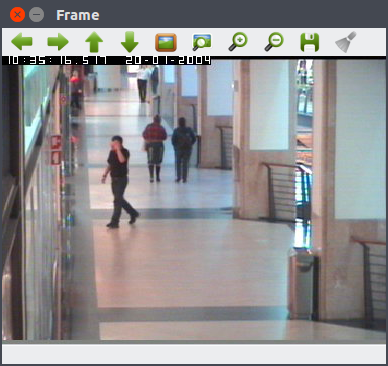
\includegraphics[width=1\linewidth]{figures/background/frame_caviar.png}
    \caption{CAVIAR}
  \end{subfigure}
  \hfill
  \begin{subfigure}{.49\linewidth}
    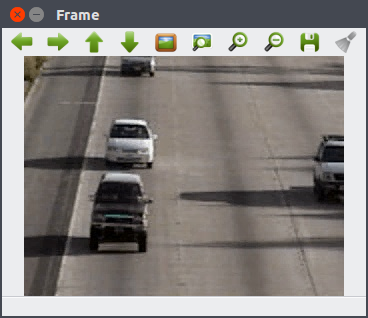
\includegraphics[width=1\linewidth]{figures/background/frame_highway1.png}
    \caption{aton\_highway1}
  \end{subfigure}
  \caption{Original dataset frames.}
\end{figure}

% vthresh default
\begin{sidewaysfigure}
  \centering
  \begin{subfigure}{.48\linewidth}
    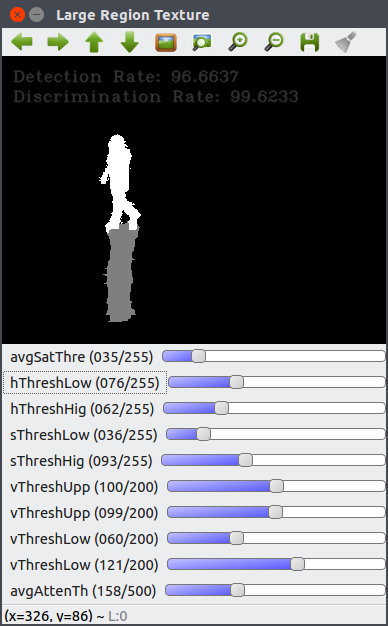
\includegraphics[width=1\linewidth]{figures/background/lr_caviar_default.png}
    \caption{}
  \end{subfigure}
  \hfill
  \begin{subfigure}{.49\linewidth}
    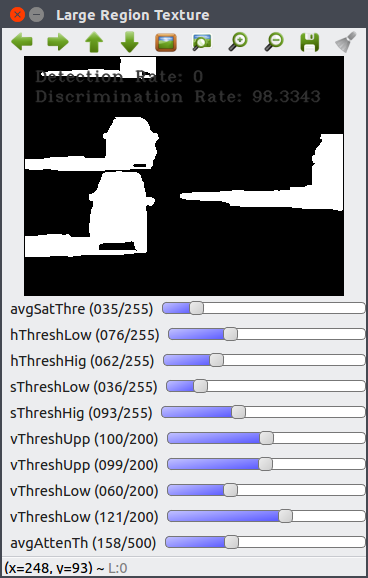
\includegraphics[width=1\linewidth]{figures/background/lr_highway1_default.png}
    \caption{}
  \end{subfigure}
  \caption{Default parameters (Datasets provided by Sanin, et al. [\ref{Sanin}]) (a) Detection: 96.6637, Discrimination: 99.6233. (b) Detection: 0, Discrimination: 98.3343}
  \label{fig:vthreshdefault}
\end{sidewaysfigure}

% vthresh15
\begin{sidewaysfigure}
  \centering
  \begin{subfigure}{.48\linewidth}
    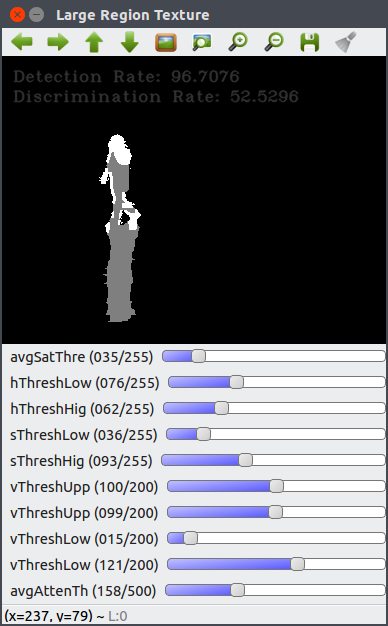
\includegraphics[width=1\linewidth]{figures/background/lr_caviar_thresh15.png}
    \caption{\textit{vThreshLower: 121}}
  \end{subfigure}
  \hfill
  \begin{subfigure}{.49\linewidth}
    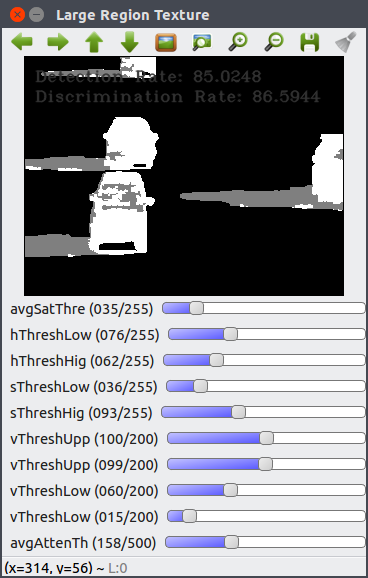
\includegraphics[width=1\linewidth]{figures/background/lr_highway1_thresh15.png}
    \caption{\textit{vThreshLower: 15}}
  \end{subfigure}
  \caption{\textit{vThreshLower} shifted from '121' to '15.' (Datasets provided by Sanin, et al. [\ref{Sanin}]) (a) Detection: 96.7076, Discrimination: 52.5296. (b) Detection: 85.0248, Discrimination: 86.5944}
  \label{fig:vthresh15}
\end{sidewaysfigure}

For a second demonstration, Geometry shadow removal was found to also showcase different results on the same scene, but with differing parameters (Figure \ref{fig:gweight}).
 
% gweight
\begin{sidewaysfigure}
  \centering
  \begin{subfigure}{.49\linewidth}
    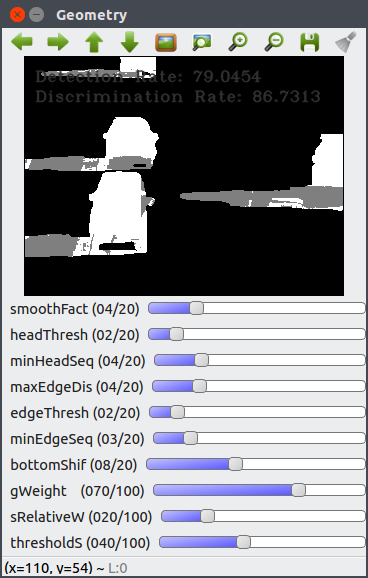
\includegraphics[width=1\linewidth]{figures/background/geo_highway1_default.png}
    \caption{\textit{gWeight: 70}}
  \end{subfigure}
  \hfill
  \begin{subfigure}{.49\linewidth}
    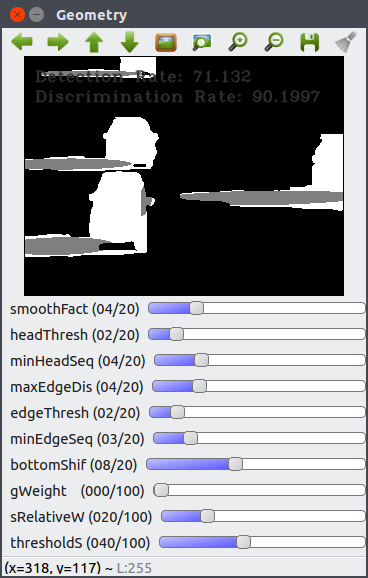
\includegraphics[width=1\linewidth]{figures/background/geo_lower_gweight.png}
    \caption{\textit{gWeight: 0}}
  \end{subfigure}
  \caption{\textit{gWeight} shifted from '70' to '0.' (a) Detection: 79.0454, Discrimination: 86.7313. (b) Detection: 71.132, Discrimination: 90.1997}
  \label{fig:gweight}
\end{sidewaysfigure}

Figure \ref{fig:vthreshdefault}, Figure \ref{fig:vthresh15} and Figure \ref{fig:gweight} demonstrate the necessity for parameter tuning to occur between environments. Each shadow removal method has been found to have hard-coded, mutable parameters that affect the shadow removal in a given environment.

%%%
\section{Research Therein, If Ye Dare}
%%%

\subsection{Objective}

No leading shadow removal methods are robust enough to compensate for a scene over time, nor are they suitable for deployment in an environment without a priori tuning of algorithm parameters. Our research seeks to establish an understanding of scene properties that affect shadow removal, and utilize that understanding to perform optimal shadow removal in an arbitrary environment. This requires the creation of an adaptive model which automatically configures a shadow removal method to optimally perform given the collected scene properties.

%The prior assumptions that are required for leading shadow removal methods to perform optimally rarely lend themselves to quantization or scalability; e.g., a geometric method exercised in this research performs optimally in situations with clearly defined upright objects with predictable shapes. Methods like this one require more of an understanding of semantic scene content rather than lower level measures such as color saturation. Therefore, the technical challenge of the proposed research lies in properly quantifying salient scene properties and content, especially in how these properties pertain to algorithmic methods such as shadow removal. The algorithmic parameters of the selected shadow removal methods can number more than 30 for a particular method. Accordingly, the proposed research requires relatively large-scale sensitivity testing for these parameters in different scenes. The large number of algorithmic parameters incites the need for identifying not only how these parameters affect shadow removal according to the scene's environment, but also how these parameters affect each other.

%Lastly, in order to create an adaptive model for shadow removal divorced of prior assumptions, the model requires an understanding of how observed environmental characteristics change over time. There is a need for adaptivity in most applications requiring shadow removal, and in the process of obtaining the diverse data sets necessary for this research, the degree to which certain scene parameters change over time can be observed.

\subsection{Approach}

We implement a proof-of-concept for adapting shadow removal to arbitrary scenes. Our adaptation model consists of selecting an algorithmic parameter, analyzing current environmental properties, and intelligently utilizing those properties to calculate a value for the selected algorithm parameter that improves shadow removal. The general flow of our methodology is represented in Figure \ref{fig:overview}. The proof-of-concept is created in eight steps:

\begin{figure}
  \centering
  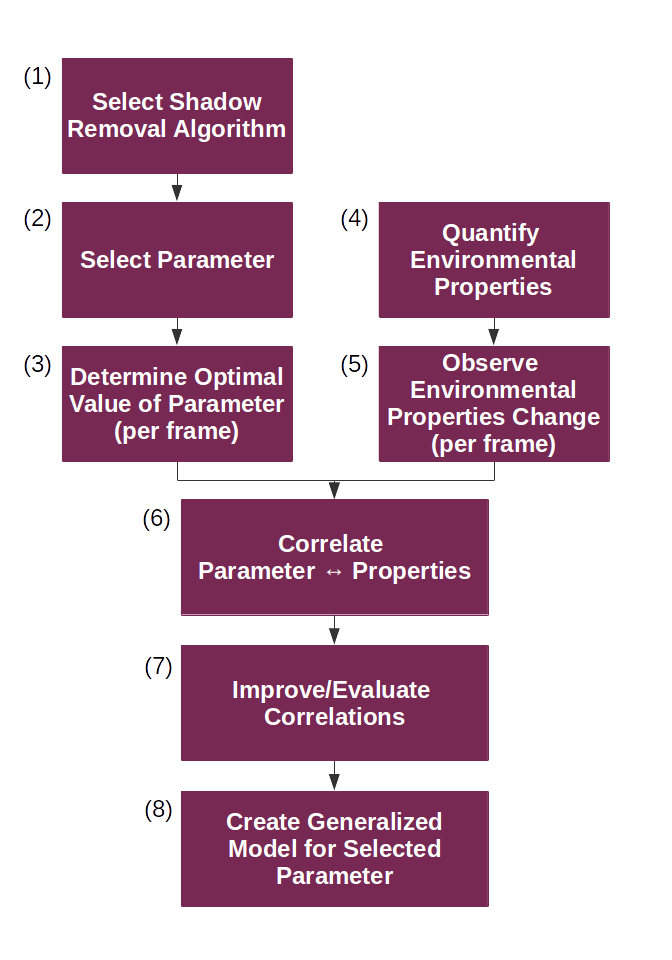
\includegraphics[width=.85\linewidth]{figures/background/overview.png}
  \caption{Proof-of-concept overview.}
  \label{fig:overview}
\end{figure}

\begin{enumerate}
\item \underline{Select Shadow Removal Algorithm}: The scope of the proof-of-concept model is restricted to one shadow removal algorithm. The algorithm selected must display reasonable sensitivity to both environmental changes. This proof-of-concept utilizes Physical shadow removal. Algorithm selection is detailed in section \ref{section:selectalgorithm}.

\item \underline{Select Parameter}: In addition to demonstrating sensitivity to environmental change, the selected algorithm must also display sensitivity to parametric change. In section \ref{section:selectparameter}, we analyze multiple candidate parameters proven to significantly affect the accuracy of shadow removal.

\item \underline{Determine Optimal Value of Parameter (per frame)}: In accordance with our selection strategy, each frame of a dataset has an optimal value for the selected parameter, i.e., there is an optimal value for which shadow removal is maximized. The process for extracting these optimal values is detailed in section \ref{section:datacollection}.

\item \underline{Quantify Scene Properties}: Observed environmental properties are the most influential factor for creating an adaptive model. Section \ref{section:envassess} details identifying and quantifying salient environmental properties. 

\item \underline{Observe Scene Properties Change (per frame)}: Our adaptive model requires that an algorithm may adapt to arbitrary environments as well as environmental changes. Environmental properties' values are recorded for each frame of a dataset.

\item \underline{Correlate Optimal Parameter Value and Environmental Properties}: By analyzing the correlation between optimal parameter values and environmental properties, we receive a quantitative understanding of how well that environmental parameter would serve as the basis for an adaptive model. For example, if our optimal parameter value increases by $x\%$ from frame 1 to frame 2, and our environmental property also increases by $x\%$ from frame 1 to frame 2, that environmental property may be used to predict an appropriate value of our algorithm parameter. Consistent correlations are sought across each dataset to eliminate false positives.

\item \underline{Improve/Evaluate Correlations}: We build our adaptive model on both direct and indirect correlations. Multiple contributing environmental properties are combined to improve correlation and thereby shadow removal. Indirect properties are evaluated in sections \ref{section:nonlinearatten}, \ref{section:brightnessmodels}, and \ref{section:lowcSIFT}.

\item \underline{Create General Model for Selected Parameter}: Incorporating direct and indirect correlative environmental properties, we construct an adaptive model capable of calculating a new value for the algorithm parameter that improves shadow removal. This model is independent of dataset, and is calculated per frame, rather than applied to every frame in a dataset. Methodology for building this model is found in section \ref{section:model}.
\end{enumerate}

\end{document}

%\section{Origin and History}
%Previous research pertaining to this research topic include research regarding shadow removal itself, threshold selection for shadow removal, scene characteristics, and scene modeling. This section will also explore the little precedent found in both intelligently selecting algorithm parameters based on scene content, and intelligently selecting between multiple shadow removal methods in a hybrid scheme.

%Characterization of a scene or environment is traditionally done with global parameters such as global hue, saturation, and value (HSV), or color variance. However, more scene properties are needed for proper identification of semantic scene content, needed for this	 research. The ‘gist’ of scene, proposed by Oliva et al. in [5], compares evaluations of the properties of scene, using low-level features and simple arrangement of volumetric forms. Similarly, in [6], Oliva et al. evaluates the content of a scene using shape modeling such as the openness, ruggedness, roughness, expansion of a scene, creating the ‘spatial envelope’ of a scene. Lowe et al. propose the scale-invariant feature transform (SIFT), which utilizes and identifies features of a scene that are robust to noise, illumination, distortion, and viewpoint [7]. Bayesian Scene Modeling, proposed by Fei-Fei et al., utilizes the ‘bag-of-words’ strategy, building a dictionary of codewords relevant to a scene via unsupervised machine learning [8]. This approach creates a ‘theme’ for a scene built upon these collected codewords, categorizing complex diverse scenes into 13 categories (highway, coast, mountain, etc). 

%There is precedent for intelligently adapting parameters for shadow removal. Sanin et al., in the implementation of Large Region Texture shadow removal, measure the average global attenuation, saturation, and foreground object perimeter of a scene. The algorithm selects several differing parameter values for hue, saturation, and value thresholds based on the average shadow attenuation and saturation of the scene. It also modifies the texture differential radius needed to qualify a pixel as shadow based on the perimeter of the foreground object in question.

%\section{Work Completed}

%The implementations of the various approaches came with hard-coded parameters that were found to be correspondent with the provided datasets. Prominent parameters include:

%There are many more mutable parameters that affect shadow removal efficacy, and again, a more complete taxonomy will be provided. 
%In order to then quickly evaluate the effect of modifying these in-built parameters, a graphical interface was created to adjust them during runtime and view the effects. The interface supports either entire sequences (e.g. video) or singular frames. The interface supports any of the aforementioned shadow removal methods. 

%Fig. 1. Graphical interface for permuting parameters.

%The graphical interface is a crucial development in terms precisely measuring each parameter's effect on a given scene. However, in order to study shadow removal in terms of adaptivity over time, a more procedural method was required. Courtesy of username ‘brofield’, SimpleINI (github.com/brofield/simpleini), licensed under MIT, allowed for creation of .ini files containing any given removal method's default parameters. The algorithms themselves were then modified to allow for runtime modifications to be made to these parameters, meaning a procedural, iterative approach to analysis was created. A python script capable of writing to this .ini file allows for rapid permutation of parameters and values.

%Develop holistic scene content understanding in order to select shadow removal method for the ‘macro’ stage of hypervisor program. A quantization of seemingly qualitative scene content is required to better select between shadow removal methods. Some of this scene content includes shadow orientation vs. foreground object orientation, pre-existing static scene shadows, foreground object classification, distinctiveness of foreground objects (color differences in particular), light source in a scene, and many more. Building up an understanding of these scene properties may also help with the ‘micro’ stage of the proposed framework.

%Develop understanding of how these scene/environment parameters change over time of day and between locales. Observation of how both the quantitative and qualitative scene parameters change over time is required to create the proposed adaptive framework. This step will be simple for things like shadow intensity and global saturation, but more difficult for aforementioned properties like static shadows and object classification.

%Create correlation between global scene/environment properties and shadow removal accuracy. This step represents the main experimental thrust of the proposed research detailed thoroughly in this research summary.

%Use the aforementioned correlation to build hypervisor program to deploy adaptive shadow removal in arbitrary scenes and environments. This will be done primarily in C++, using the OpenCV API.

